\chapter{Future Colliders}
\label{chapter:colliders}

\epigraph{Progress is not a straight line.}{An Wang}

In the post-LHC era, the major unanswered questions in particle physics centre around the Higgs boson and its properties, the identification of additional sources of CP-violation that can account for the universe's abundance of matter and paucity of antimatter, and the discovery of physics beyond the Standard Model. There are many investigations into each of these fields that utilise the Large Hadron Collider, or will leverage the upgrades for the \acrfull{HL-LHC}. However, now that the Higgs boson has been identified successfully, one of the most fruitful avenues for further research is the construction and operation of a lepton collider with sufficient centre-of-mass energy to produce Higgs bosons in larger numbers.

The search for higher precision on the Higgs, as well as for new physics in that regime, are the primary motivations for the construction of future collider experiments, especially lepton colliders, to succeed the Large Hadron Collider. There are several proposals for future lepton colliders, which are broadly separated into two groups. There are the linear colliders, using two accelerator arms with the interaction point in the centre. The main candidates for this style of collider are the \acrfull{ILC} and the \acrfull{CLIC}. There are also the circular colliders, similar in structure to the Large Hadron Collider, with multiple interaction points placed around the ring. The main candidates for circular colliders are \acrfull{FCC} and \acrfull{CEPC}. 

All of these proposed colliders share many features, design considerations and challenges, as does the on-going international effort in research and development to make these colliders a reality. [...]

\section{The physics case for a lepton collider}
[...]

This follows a historical pattern in physics -- as the energy frontier advances, hadron colliders are used to discover new physics and new phenomena followed by lepton colliders to establish these phenomena in greater detail and precision. [...]

[...]

Measurements of particles and their properties will be made significantly easier and thus more precise in the final state environment of a lepton collider -- using fundamental particles removes the need to consider parton distribution functions in the collision, or to account for the ``particle shrapnel'' produced by the collision and received in the detectors. This cleaner environment allows for precision measurements of the Standard Model, putting better constaints on new physics. It will also allow high-precision measurements of the properties of the Higgs boson, allowing lepton colliders to determine their properties very precisely. Many BSM models rely upon Higgs bosons that differ from those predicted by the Standard Model, or additional Higgs states, and a higher sensitivity in this regime will allow better limits on these models. 

\begin{table}[h]
\centering
	\begin{tabular}{ c | c | c }
	\hline \hline
	\textbf{Energy} & \textbf{Reaction} & \textbf{Physics goal} \\ \hline
	 91 GeV & $e^+ e^- \rightarrow Z$ & ultra-precision electroweak \\ \hline
	 160 GeV & $e^+ e^- \rightarrow WW$ & ultra-precision W mass \\ \hline
	 250 GeV & $e^+ e^- \rightarrow Zh$ & precision Higgs coupling \\ \hline
	 350-500 GeV & $e^+ e^- \rightarrow t\overline{t}$ & top quark mass and couplings \\
	   & $e^+ e^- \rightarrow WW$ & precision W coupling \\
	   & $e^+ e^- \rightarrow \nu \overline{\nu} h$ & precision Higgs coupling \\ \hline
	 500 GeV & $e^+ e^- \rightarrow f \overline{f}$ & precision search for Z' \\
	   & $e^+ e^- \rightarrow t \overline{t}h$ & Higgs coupling to top \\
	   & $e^+ e^- \rightarrow Zhh$ & Higgs self-coupling \\
	   & $e^+ e^- \rightarrow \widetilde{\chi} \widetilde{\chi}$ & search for supersymmetry \\
	   & $e^+ e^- \rightarrow AH, H^+, H^-$ & search for extended Higgs states \\ \hline
	 700-1000 GeV & $e^+ e^- \rightarrow \nu \overline{\nu} hh$ & Higgs self-coupling \\
	   & $e^+ e^- \rightarrow \nu \overline{\nu} VV$ & composite Higgs sector \\
	   & $e^+ e^- \rightarrow  \nu \overline{\nu} t \overline{t}$ & composite Higgs and top \\
	   & $e^+ e^- \rightarrow \tilde{t} \tilde{t}^*$ & search for supersymmetry \\ \hline
	\end{tabular}
	\caption{Physics processes of interest at lepton colliders across various energies.}
	\label{table:colliders/physics-goals}
\end{table}

[...]

\section{The International Linear Collider}
The \acrfull{ILC} is a proposed high-luminosity linear electron-positron collider based upon 1.3GHz superconducting radio frequency (SCRF) accelerating technology. The centre of mass energy ($$\sqrt{s}$$) would be 250 GeV, upgradable to 500 GeV and then to 1 TeV at a later date. The total footprint of the complex would be 31km in length, with the arms using magnets with an accelerating gradient of 31.5 MVm\^{-1} in metre-long superconducting nine-cell niobium cavities operating at 2K.

The ILC and its detectors are designed with the intention of becoming a "Higgs factory" -- producing large numbers of Higgs bosons to allow more detailed study of these particles.

There were a number of proposed sites for the ILC, including CERN in Geneva, DESY in Hamburg, and \acrshort{JINR} near Moscow. Due to the 2008 economic crisis, the United States and United Kingdom severely cut funding for linear collider projects, and this resulted in Japan seeking to make a proposal to host the collider in the Kitakami Highlands region of Iwate prefecture. 

A report from the Science Council of Japan (a representative organisation of the Japanese science community) released in early 2019 expressed that they had not reached a consensus as to whether to support hosting the ILC in Japan. Some  of the reasons cited were concerns over international cost-sharing in the long-term, as well as whether the expected scientific outcomes would justify the unprecedented human resource requirements and infrastructure necessary to make the ILC a reality \cite{linearcolliders-scj-report}.

%Reference (24/04/2019): http://www.linearcollider.org/content/decision-international-linear-collider-“not-what-we-had-hoped-progress-nevertheless” 
On 7th March 2019, the Japanese government expressed that it would not make a proposal to host the collider in Japan. The Japanese government did however express interest in the ILC, and declared that it would be continuing discussion and interest in the project as a whole.

[...]

\subsection{The ILD and SiD detectors}
[...]

One of the unique features of the ILC is the push-pull detector system. This is a moving platform in the chamber housing the interaction point, upon which two detectors can be mounted. The platform can be moved to change which detector is in the beamline, allowing a linear collider to function with multiple detectors. Switching detectors is expected to take [some] hours. This allows the two detectors to specialise for different physics studies and goals, much like the experiments at the Large Hadron Collider at CERN, which is normally not possible with linear colliders. [?] [...]

\subsubsection{The International Large Detector (ILD)}
[...]

The finished ILD will weigh 14,000 metric tonnes, and using a magnetic field of 3.5 Tesla will offer a spatial resolution of 3 microns in the vertex tracker, and 60 microns in the central TPC tracker. 

\begin{figure}[h]
	\centering
	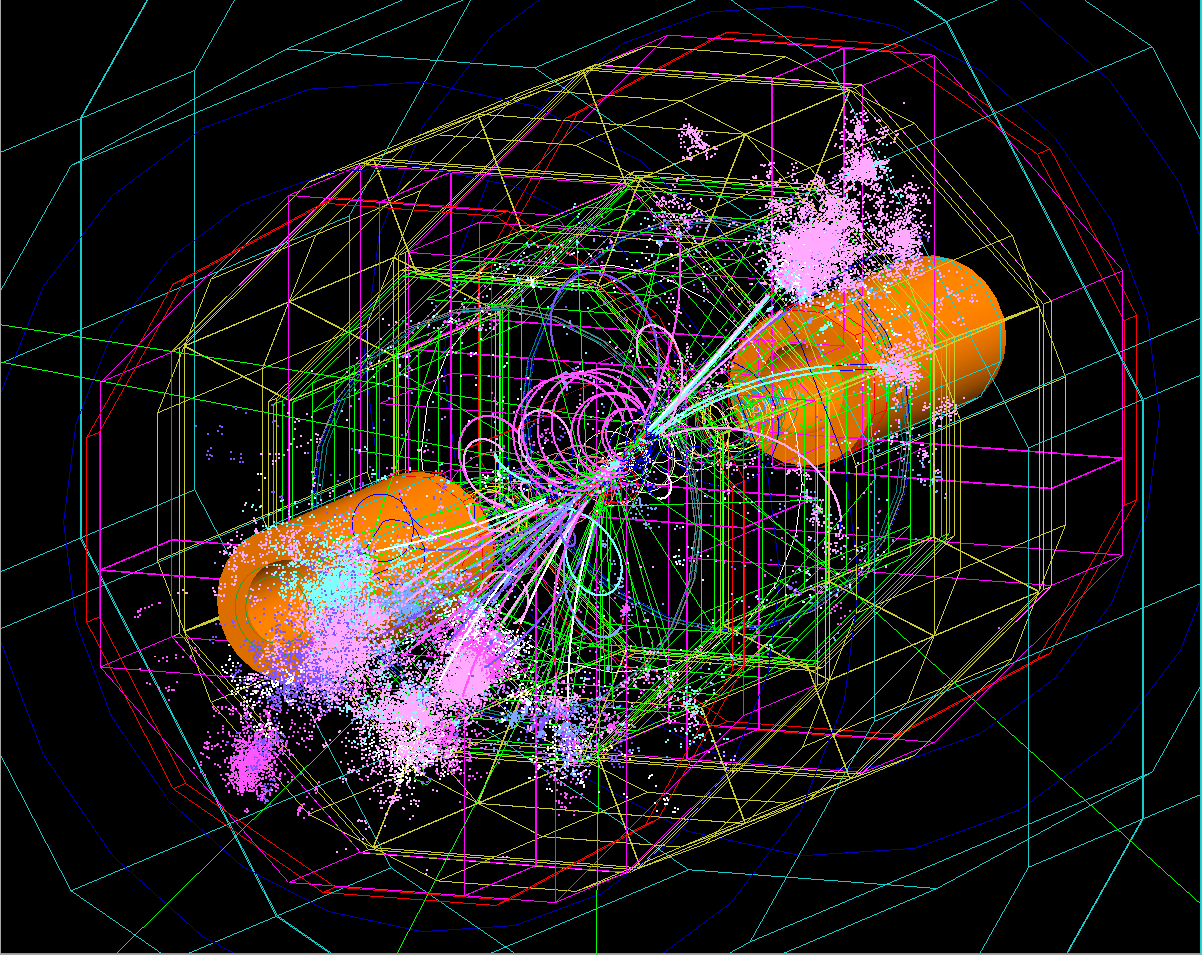
\includegraphics[width=0.75\textwidth]{../Pictures/SimulatedEvent1.png}
	\caption{Visualisation of a simulated tth event in the ILD. Charged particles can be easily identified by their curved, coiled or spiral paths, and the jets are clearly visible as the light pink and purple areas near the beampipes on either side.}
	\label{figure:colliders/ILD/tth-simulation}
\end{figure}

\subsubsection{The Silicon Detector (SiD)}
[...]

\section{The Compact Linear Collider}
[...]

The CLIC project foresees a programme spanning 22 years, over which multiple upgrades to the centre-of-mass energy would take place. Initial construction would be at 380 GeV, focusing on precision measurements of top-quark and Higgs physics. Further upgrades would increase the centre-of-mass energy to 1.5 TeV, then finally 3 GeV. Physics goals in these later stages would involve searches for new physics processes, as well as precision measurements of rare Higgs processes, and of new states discovered at the LHC or earlier stages of CLIC. 

[...] CLIC would be built beneath the existing LHC ring at CERN, stretching across the French-Swiss border and running parallel to the feet of the Jura mountain range. This placement is determined by the geological features of the region around Geneva and the feet of the Juras, [...]


[...]

As of writing, the CLIC project has been submitted as input for the European Particle Physics Strategy Update, which will decide which projects the CERN collaboration chooses to pursue from 2020  onwards. [...]

CLIC's initial centre-of-mass energy will be 380 GeV, with successive upgrades increasing this to 1.5 TeV and finally 3 TeV. 

\section{The Future Circular Collider}
The \acrfull{FCC} is a series of concepts for a future collider that would be located in the Geneva area near the existing LHC ring. The FCC project as a whole has three different accelerator concepts -- the FCC-hh for proton/proton and ion/ion collisions, the FCC-ee for electron/positron collisions, and the FCC-he for electron/proton collisions.

The initial proposal is to construct a circular electron/positron collider -- the FCC-ee -- with a circumference of 100km and delivering a maximum centre-of-mass energy of 365 GeV. The motivation for this is that at this energy range -- the electroweak scale -- the FCC would be able to access the Z pole, the W- and top-pair production thresholds, as well as producing a large number of Higgs bosons. 

A further part of the proposal for the FCC is that following the conclusion of the physics programme of the FCC-ee, the tunnels constructed to house the accelerator would be re-used for the FCC-hh, a hadron collider. This follows a similar use case as the LHC, which re-purposed the tunnels used for the \acrfull{LEP}. It is claimed that the FCC-hh built in these tunnels would be able to reach centre-of-mass energies of at least 100 TeV.

According to the given timeline, the FCC-ee would begin construction in 2028, and first physics would take place in 2039. 


[...]

\section{The Circular Electron Positron Collider}

The \acrfull{CEPC} is a proposal for a circular electron-positron collider 

[...]